% Created by tikzDevice version 0.12.6 on 2026-05-17 11:16:31
% !TEX encoding = UTF-8 Unicode
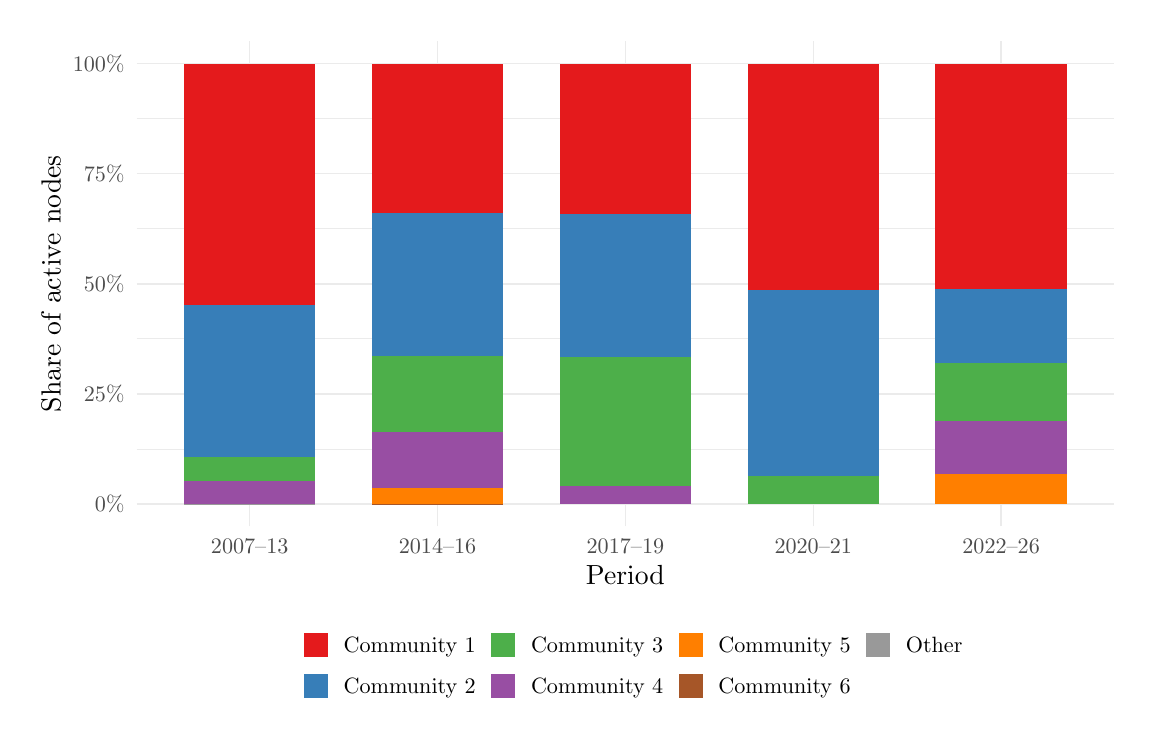
\begin{tikzpicture}[x=1pt,y=1pt]
\definecolor{fillColor}{RGB}{255,255,255}
\path[use as bounding box,fill=fillColor,fill opacity=0.00] (0,0) rectangle (397.48,252.94);
\begin{scope}
\path[clip] (  0.00,  0.00) rectangle (397.48,252.94);
\definecolor{fillColor}{RGB}{255,255,255}

\path[fill=fillColor] (  0.00, -0.00) rectangle (397.48,252.94);
\end{scope}
\begin{scope}
\path[clip] ( 39.49, 72.81) rectangle (392.48,247.95);
\definecolor{drawColor}{gray}{0.92}

\path[draw=drawColor,line width= 0.3pt,line join=round] ( 39.49,100.67) --
	(392.48,100.67);

\path[draw=drawColor,line width= 0.3pt,line join=round] ( 39.49,140.48) --
	(392.48,140.48);

\path[draw=drawColor,line width= 0.3pt,line join=round] ( 39.49,180.28) --
	(392.48,180.28);

\path[draw=drawColor,line width= 0.3pt,line join=round] ( 39.49,220.08) --
	(392.48,220.08);

\path[draw=drawColor,line width= 0.5pt,line join=round] ( 39.49, 80.77) --
	(392.48, 80.77);

\path[draw=drawColor,line width= 0.5pt,line join=round] ( 39.49,120.58) --
	(392.48,120.58);

\path[draw=drawColor,line width= 0.5pt,line join=round] ( 39.49,160.38) --
	(392.48,160.38);

\path[draw=drawColor,line width= 0.5pt,line join=round] ( 39.49,200.18) --
	(392.48,200.18);

\path[draw=drawColor,line width= 0.5pt,line join=round] ( 39.49,239.98) --
	(392.48,239.98);

\path[draw=drawColor,line width= 0.5pt,line join=round] ( 80.22, 72.81) --
	( 80.22,247.95);

\path[draw=drawColor,line width= 0.5pt,line join=round] (148.11, 72.81) --
	(148.11,247.95);

\path[draw=drawColor,line width= 0.5pt,line join=round] (215.99, 72.81) --
	(215.99,247.95);

\path[draw=drawColor,line width= 0.5pt,line join=round] (283.87, 72.81) --
	(283.87,247.95);

\path[draw=drawColor,line width= 0.5pt,line join=round] (351.76, 72.81) --
	(351.76,247.95);
\definecolor{fillColor}{RGB}{55,126,184}

\path[fill=fillColor] ( 56.46, 97.97) rectangle (103.98,152.83);
\definecolor{fillColor}{RGB}{77,175,74}

\path[fill=fillColor] ( 56.46, 89.13) rectangle (103.98, 97.97);
\definecolor{fillColor}{RGB}{228,26,28}

\path[fill=fillColor] ( 56.46,152.83) rectangle (103.98,239.98);
\definecolor{fillColor}{RGB}{152,78,163}

\path[fill=fillColor] ( 56.46, 80.84) rectangle (103.98, 89.13);
\definecolor{fillColor}{RGB}{255,127,0}

\path[fill=fillColor] ( 56.46, 80.83) rectangle (103.98, 80.84);
\definecolor{fillColor}{RGB}{166,86,40}

\path[fill=fillColor] ( 56.46, 80.81) rectangle (103.98, 80.83);
\definecolor{fillColor}{gray}{0.60}

\path[fill=fillColor] ( 56.46, 80.77) rectangle (103.98, 80.81);
\definecolor{fillColor}{RGB}{152,78,163}

\path[fill=fillColor] (124.35, 86.54) rectangle (171.87,106.71);
\definecolor{fillColor}{RGB}{77,175,74}

\path[fill=fillColor] (124.35,106.71) rectangle (171.87,134.44);
\definecolor{fillColor}{RGB}{255,127,0}

\path[fill=fillColor] (124.35, 80.78) rectangle (171.87, 86.54);
\definecolor{fillColor}{RGB}{55,126,184}

\path[fill=fillColor] (124.35,134.44) rectangle (171.87,185.86);
\definecolor{fillColor}{RGB}{228,26,28}

\path[fill=fillColor] (124.35,185.86) rectangle (171.87,239.98);
\definecolor{fillColor}{RGB}{166,86,40}

\path[fill=fillColor] (124.35, 80.77) rectangle (171.87, 80.78);
\definecolor{fillColor}{RGB}{152,78,163}

\path[fill=fillColor] (192.23, 80.77) rectangle (239.75, 87.32);
\definecolor{fillColor}{RGB}{77,175,74}

\path[fill=fillColor] (192.23, 87.32) rectangle (239.75,134.10);
\definecolor{fillColor}{RGB}{55,126,184}

\path[fill=fillColor] (192.23,134.10) rectangle (239.75,185.71);
\definecolor{fillColor}{RGB}{228,26,28}

\path[fill=fillColor] (192.23,185.71) rectangle (239.75,239.98);
\definecolor{fillColor}{RGB}{55,126,184}

\path[fill=fillColor] (260.11, 90.79) rectangle (307.63,158.27);
\definecolor{fillColor}{RGB}{228,26,28}

\path[fill=fillColor] (260.11,158.27) rectangle (307.63,239.98);
\definecolor{fillColor}{RGB}{77,175,74}

\path[fill=fillColor] (260.11, 80.77) rectangle (307.63, 90.79);

\path[fill=fillColor] (328.00,110.92) rectangle (375.51,131.67);
\definecolor{fillColor}{RGB}{255,127,0}

\path[fill=fillColor] (328.00, 80.77) rectangle (375.51, 91.68);
\definecolor{fillColor}{RGB}{55,126,184}

\path[fill=fillColor] (328.00,131.67) rectangle (375.51,158.61);
\definecolor{fillColor}{RGB}{152,78,163}

\path[fill=fillColor] (328.00, 91.68) rectangle (375.51,110.92);
\definecolor{fillColor}{RGB}{228,26,28}

\path[fill=fillColor] (328.00,158.61) rectangle (375.51,239.98);
\end{scope}
\begin{scope}
\path[clip] (  0.00,  0.00) rectangle (397.48,252.94);
\definecolor{drawColor}{gray}{0.30}

\node[text=drawColor,anchor=base east,inner sep=0pt, outer sep=0pt, scale=  0.80] at ( 34.99, 78.02) {0\%};

\node[text=drawColor,anchor=base east,inner sep=0pt, outer sep=0pt, scale=  0.80] at ( 34.99,117.82) {25\%};

\node[text=drawColor,anchor=base east,inner sep=0pt, outer sep=0pt, scale=  0.80] at ( 34.99,157.62) {50\%};

\node[text=drawColor,anchor=base east,inner sep=0pt, outer sep=0pt, scale=  0.80] at ( 34.99,197.43) {75\%};

\node[text=drawColor,anchor=base east,inner sep=0pt, outer sep=0pt, scale=  0.80] at ( 34.99,237.23) {100\%};
\end{scope}
\begin{scope}
\path[clip] (  0.00,  0.00) rectangle (397.48,252.94);
\definecolor{drawColor}{gray}{0.30}

\node[text=drawColor,anchor=base,inner sep=0pt, outer sep=0pt, scale=  0.80] at ( 80.22, 62.80) {2007--13};

\node[text=drawColor,anchor=base,inner sep=0pt, outer sep=0pt, scale=  0.80] at (148.11, 62.80) {2014--16};

\node[text=drawColor,anchor=base,inner sep=0pt, outer sep=0pt, scale=  0.80] at (215.99, 62.80) {2017--19};

\node[text=drawColor,anchor=base,inner sep=0pt, outer sep=0pt, scale=  0.80] at (283.87, 62.80) {2020--21};

\node[text=drawColor,anchor=base,inner sep=0pt, outer sep=0pt, scale=  0.80] at (351.76, 62.80) {2022--26};
\end{scope}
\begin{scope}
\path[clip] (  0.00,  0.00) rectangle (397.48,252.94);
\definecolor{drawColor}{RGB}{0,0,0}

\node[text=drawColor,anchor=base,inner sep=0pt, outer sep=0pt, scale=  1.00] at (215.99, 51.86) {Period};
\end{scope}
\begin{scope}
\path[clip] (  0.00,  0.00) rectangle (397.48,252.94);
\definecolor{drawColor}{RGB}{0,0,0}

\node[text=drawColor,rotate= 90.00,anchor=base,inner sep=0pt, outer sep=0pt, scale=  1.00] at ( 11.89,160.38) {Share of active nodes};
\end{scope}
\begin{scope}
\path[clip] (  0.00,  0.00) rectangle (397.48,252.94);
\definecolor{fillColor}{RGB}{228,26,28}

\path[fill=fillColor] ( 99.84, 25.61) rectangle (108.50, 34.27);
\end{scope}
\begin{scope}
\path[clip] (  0.00,  0.00) rectangle (397.48,252.94);
\definecolor{fillColor}{RGB}{55,126,184}

\path[fill=fillColor] ( 99.84, 10.65) rectangle (108.50, 19.31);
\end{scope}
\begin{scope}
\path[clip] (  0.00,  0.00) rectangle (397.48,252.94);
\definecolor{fillColor}{RGB}{77,175,74}

\path[fill=fillColor] (167.56, 25.61) rectangle (176.23, 34.27);
\end{scope}
\begin{scope}
\path[clip] (  0.00,  0.00) rectangle (397.48,252.94);
\definecolor{fillColor}{RGB}{152,78,163}

\path[fill=fillColor] (167.56, 10.65) rectangle (176.23, 19.31);
\end{scope}
\begin{scope}
\path[clip] (  0.00,  0.00) rectangle (397.48,252.94);
\definecolor{fillColor}{RGB}{255,127,0}

\path[fill=fillColor] (235.29, 25.61) rectangle (243.95, 34.27);
\end{scope}
\begin{scope}
\path[clip] (  0.00,  0.00) rectangle (397.48,252.94);
\definecolor{fillColor}{RGB}{166,86,40}

\path[fill=fillColor] (235.29, 10.65) rectangle (243.95, 19.31);
\end{scope}
\begin{scope}
\path[clip] (  0.00,  0.00) rectangle (397.48,252.94);
\definecolor{fillColor}{gray}{0.60}

\path[fill=fillColor] (303.01, 25.61) rectangle (311.68, 34.27);
\end{scope}
\begin{scope}
\path[clip] (  0.00,  0.00) rectangle (397.48,252.94);
\definecolor{drawColor}{RGB}{0,0,0}

\node[text=drawColor,anchor=base west,inner sep=0pt, outer sep=0pt, scale=  0.80] at (114.15, 27.18) {Community 1};
\end{scope}
\begin{scope}
\path[clip] (  0.00,  0.00) rectangle (397.48,252.94);
\definecolor{drawColor}{RGB}{0,0,0}

\node[text=drawColor,anchor=base west,inner sep=0pt, outer sep=0pt, scale=  0.80] at (114.15, 12.22) {Community 2};
\end{scope}
\begin{scope}
\path[clip] (  0.00,  0.00) rectangle (397.48,252.94);
\definecolor{drawColor}{RGB}{0,0,0}

\node[text=drawColor,anchor=base west,inner sep=0pt, outer sep=0pt, scale=  0.80] at (181.88, 27.18) {Community 3};
\end{scope}
\begin{scope}
\path[clip] (  0.00,  0.00) rectangle (397.48,252.94);
\definecolor{drawColor}{RGB}{0,0,0}

\node[text=drawColor,anchor=base west,inner sep=0pt, outer sep=0pt, scale=  0.80] at (181.88, 12.22) {Community 4};
\end{scope}
\begin{scope}
\path[clip] (  0.00,  0.00) rectangle (397.48,252.94);
\definecolor{drawColor}{RGB}{0,0,0}

\node[text=drawColor,anchor=base west,inner sep=0pt, outer sep=0pt, scale=  0.80] at (249.60, 27.18) {Community 5};
\end{scope}
\begin{scope}
\path[clip] (  0.00,  0.00) rectangle (397.48,252.94);
\definecolor{drawColor}{RGB}{0,0,0}

\node[text=drawColor,anchor=base west,inner sep=0pt, outer sep=0pt, scale=  0.80] at (249.60, 12.22) {Community 6};
\end{scope}
\begin{scope}
\path[clip] (  0.00,  0.00) rectangle (397.48,252.94);
\definecolor{drawColor}{RGB}{0,0,0}

\node[text=drawColor,anchor=base west,inner sep=0pt, outer sep=0pt, scale=  0.80] at (317.32, 27.18) {Other};
\end{scope}
\end{tikzpicture}
